% Opcje klasy 'iithesis' opisane sa w komentarzach w pliku klasy. Za ich pomoca
% ustawia sie przede wszystkim jezyk i rodzaj (lic/inz/mgr) pracy, oraz czy na
% drugiej stronie pracy ma byc skladany wzor oswiadczenia o autorskim wykonaniu.
\documentclass[polish,shortabstract,inz]{iithesis}

\usepackage[utf8]{inputenc}

%%%%% DANE DO STRONY TYTUŁOWEJ
% Niezaleznie od jezyka pracy wybranego w opcjach klasy, tytul i streszczenie
% pracy nalezy podac zarowno w jezyku polskim, jak i angielskim.
% Pamietaj o madrym (zgodnym z logicznym rozbiorem zdania oraz estetyka) recznym
% zlamaniu wierszy w temacie pracy, zwlaszcza tego w jezyku pracy. Uzyj do tego
% polecenia \fmlinebreak.
\polishtitle{Projekt i implementacja biblioteki ułatwiającej tworzenie\fmlinebreak inteligentnych agentów grających w gry planszowe}
\englishtitle{Python module to support creating AI for board games -- design and implementation}
\polishabstract{
Praca przedstawia bibliotekę ułatwiającą tworzenie inteligentnych agentów grających w gry planszowe.
Przede wszystkim jest tutaj wytłumaczone jak wygodnie używać tej biblioteki do tworzenia dwuosobowych gier planszowych z pełną informacją, bez elementu losowości.
Aby ten cel został osiągnięty praca ta w pierwszej kolejności zapewnia niezbędne wprowadzenie teoretyczne.
Kolejno zostają omówione gry planszowe takie jak: kółko i krzyżyk, connect four, lis i gęsi oraz reversi.
Gry te zostały zaimplementowane i pełnią rolę reprezentacyjną użycia biblioteki.
}
\englishabstract{
This dissertation describes Python module to support creating AI for board games.
Chapters such as theoretical introduction, examples and explanations how to write programs with that module are provided.
In support of explanations, games such as tic-tac-toe, connect four, otello, fox games have been written.
Above games have been written with carrying about clear, easy to understand code.
}
% w pracach wielu autorow nazwiska mozna oddzielic poleceniem \and
\author{Mikołaj Kowalik}
% w przypadku kilku promotorow, lub koniecznosci podania ich afiliacji, linie
% w ponizszym poleceniu mozna zlamac poleceniem \fmlinebreak
\advisor        {dr Paweł Rychlikowski}
%\date          {15.01.2019}                     % Data zlozenia pracy
% Dane do oswiadczenia o autorskim wykonaniu
\transcriptnum  {283476}                     % Numer indeksu
%\advisorgen    {dr. Pawła Rychlikowskiego} % Nazwisko promotora w dopelniaczu
%%%%%

%%%%% WLASNE DODATKOWE PAKIETY
%
%\usepackage{graphicx,listings,amsmath,amssymb,amsthm,amsfonts,tikz}
%
\usepackage{url}
\usepackage{graphicx}
\usepackage{float}
\usepackage{listings}
\lstset
{
    language=Python,
    basicstyle=\footnotesize,
    numbers=left,
    stepnumber=1,
    showstringspaces=false,
    tabsize=4,
    breaklines=true,
    breakatwhitespace=false,
}
%%%%% WŁASNE DEFINICJE I POLECENIA
%
%\theoremstyle{definition} \newtheorem{definition}{Definition}[chapter]
%\theoremstyle{remark} \newtheorem{remark}[definition]{Observation}
%\theoremstyle{plain} \newtheorem{theorem}[definition]{Theorem}
%\theoremstyle{plain} \newtheorem{lemma}[definition]{Lemma}
%\renewcommand \qedsymbol {\ensuremath{\square}}
% ...
%%%%%

\begin{document}

%%%%% POCZĄTEK ZASADNICZEGO TEKSTU PRACY

\chapter{Wprowadzenie}
Jednym z naturalnych miejsc do testowania sztucznej inteligencji są gry planszowe.
Z tego powodu pewną część przedmiotu sztuczna inteligencja stanowi implementowanie dużej liczby gier planszowych -- głównie w celach testowania algorytmów.
Celem tej pracy jest wyjście naprzeciw potrzebom, jakie powstały podczas tamtego kursu -- przekazanie odpowiedniego modułu napisanego w Pythonie programiście, który stoi przed podobnym wyzwaniem.
Tak więc, podstawowym celem tej pracy jest zapoznanie użytkownika-programisty z obsługą tytułowej biblioteki -- która ma ułatwić pewne powtarzalne czynności -- z jakimi trzeba się zmierzyć podczas pisania gry planszowej z inteligentnym, komputerowym graczem.
Praca ta zawiera następujące rozdziały:
\begin{itemize}
  \item Wprowadzenie teoretyczne -- przewidziane dla osób, które chcą poznać różnice pomiędzy algorytmami przeszukiwania (MiniMax~\cite{aibook,wazniak}, Alpha-Beta~\cite{aibook,wazniak}, MCTS~\cite{mcts1}).
  \item Rozdział poświęcony opisowi i przykładom użycia biblioteki -- znaleźć tu można podrozdziały takie jak:
    \begin{itemize}
      \item Opis środowiska uruchomieniowego.
      \item Omówienie zawartości biblioteki.
      \item Omówienie zasad gier planszowych pojawiających się w pracy.
      \item Omówienie fragmentów kodu, kluczowych z punktu widzenia użytkownika.
      \item Propozycje dalszego rozwoju biblioteki -- zostały tam przedstawione liczne propozycje usprawnień oraz rozbudowy tej biblioteki.
    \end{itemize}
  \item Zakończenie -- krótkie podsumowanie całości pracy.
\end{itemize}

W prac tej jak widać większość dotyczy praktycznego pisania programów z użyciem biblioteki.
Takie podejście zostało wybrane ze względu na to, że jest to podstawowy cel, a implementowane na potrzeby tej pracy algorytmy nie są niczym nowym -- zostały omówione już w wielu innych pracach.

Po tym krótkim wprowadzeniu przejdziemy teraz do zapowiadanego wcześniej wprowadzenia teoretycznego.


\chapter{Wprowadzenie teoretyczne}
\section{Sztuczna inteligencja a gry}
Od samego początku istnienia sztucznej inteligencji, gry planszowe były dla niej naturalnym miejscem do testowania i rozwoju.
Dobrym tego dowodem jest, że już w 1951 r. Alan Turing, nie mając dostępu do odpowiedniego komputera napisał program, którego celem było granie w szachy.

Sztuczna inteligencja w grach zawsze wzbudzała duże emocje.
Szczególnie, gdy gracze uznawani za najlepszych w swoich czasach w danych grach zostawali pokonywani.
Przykłady takich wydarzeń to:
\begin{itemize}
    \item Pierwsza wygrana komputera Deep Blue\cite{deepblue} z ówczesnym szachowym mistrzem świata Garri Kasparowem
    \item W 2015r. światowej klasy zawodnik w Go, Lee Sedol, przegrywa ze sztuczną inteligencją AlphaGo\cite{alphago} (od firmy DeepMind)
\end{itemize}

Istnieje jeszcze wiele przykładów sukcesów sztucznej inteligencji nad człowiekiem (np. warcaby), jednak ze względu na cel tej pracy reszta przykładów została pominięta.

Teraz zostanie powiedziane o problemie wyboru ruchu w grach planszowych z perspektywy sztucznej inteligencji.

\section{Problem przeszukiwania w grach planszowych}
Jednym z podstawowych problemów gier planszowych jest problem przeszukiwania.
Biblioteka skupia się na pomocy programiście poradzenia sobie właśnie z tym problemem, ale nie tylko.
Na potrzeby tej pracy wybrano trzy algorytmy przeszukiwania: MiniMax, Alpha-Beta oraz Monte Carlo Tree Search, które, od strony praktycznej, omówione są w tym wprowadzeniu.

\section{Drzewo gry}
Zanim jednak zostaną opisane algorytmy, warto jednak opisać sposób patrzenia na rozgrywkę w dowolną grę planszową (z adwersarzem), jako na drzewo możliwych ruchów.

Drzewo gry to sposób prezentacji rozgrywki.
W wierzchołkach tego drzewa znajdują się stany gry.
Dzieci wierzchołka to wszystkie możliwe do wykonania ruchy ze stanu gry, który ten wierzchołek sobą reprezentuje.
Rysunek \ref{fig:oxTree} przedstawia takie drzewa dla gry w kółko i krzyżyk.


\begin{figure}[H]
  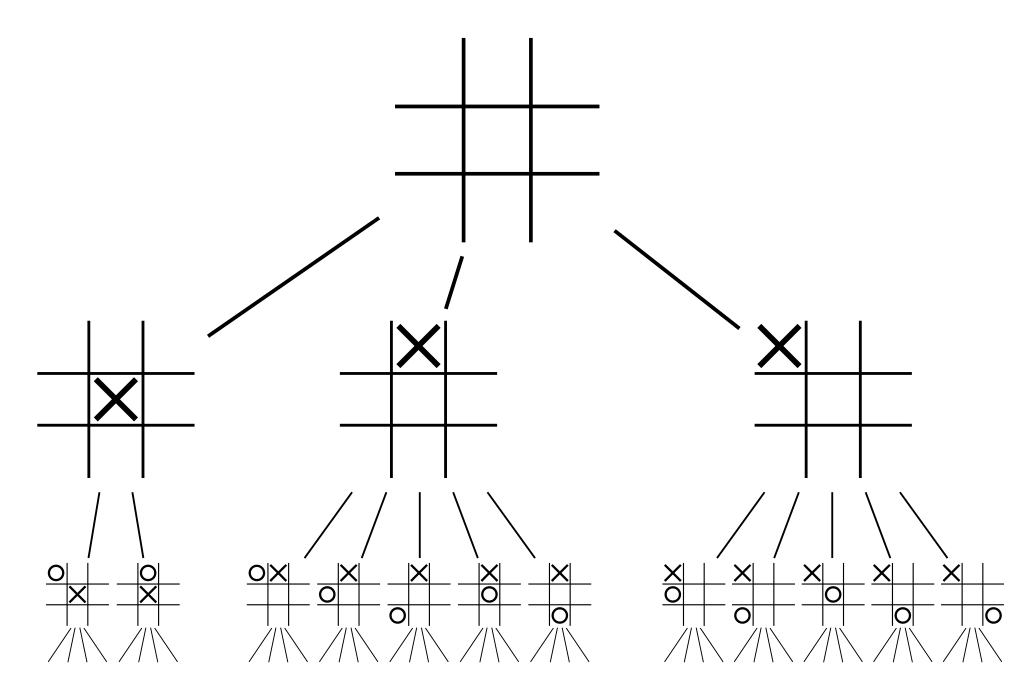
\includegraphics[scale=0.3]{./images/tictactoetree.png}
  \centering
  \caption{kółko i krzyżyk -- drzewo gry. \newline Źródło:\,\url{https://upload.wikimedia.org/wikipedia/commons/d/da/Tic-tac-toe-game-tree.svg}}
  \label{fig:oxTree}
\end{figure}

Przy tak rozumianym drzewie gry, problem wyboru ruchu sprowadza się do problemu przeszukiwania.
Jednak w odróżnienia do zwykłego przeszukiwania problemem jest przeciwnik -- o którym możemy poczynić jedynie niewielkie założenia.
Jednym z rozsądnych założeń jest przyjęcie, że przeciwnik zawsze będzie wybierał najlepszy dla siebie ruch.
Na takim założeniu opiera się właśnie algorytm MiniMax, które będzie teraz omówiony.


\section{Algorytm MiniMax}
\subsection{Pełny algorytm MiniMax}
Algorytm MiniMax w podstawowej wersji (pełny MiniMax) przegląda wszystkie możliwe ruchy i buduje całe drzewo gry.
Algorytm ten zakłada, że zarówno gracz jak i przeciwnik będą wykonywać najlepsze dla siebie ruchy.
Na podstawie tak zbudowanego drzewa gry algorytm wybiera najlepszy możliwy ruch.
Poniżej algorytm ten zapisany w postaci pseudokodu:

\bigskip
\lstinputlisting{./minimax.pseudocode}

Funkcja max\textunderscore from\textunderscore next\textunderscore state\textunderscore list zwraca maksimum z listy krotek (wartość, kolejny\textunderscore stan) -- szuka (w liście o nazwie res) maksymalnej wartości (najlepszej oceny stanu), i zwraca odpowiadającą jej krotkę (wartość, stan).
W implementacji tego algorytmu wartości win\textunderscore value, draw\textunderscore value, lost\textunderscore value -- mają odpowiednio wartości \( +\infty \), \( 0 \), \( -\infty \).
Wartości te mówią jak bardzo dany stan jest pożądany z punktu widzenia gracza player, gdzie \( +\infty \) oznacza najlepszy stan, z kolei \( -\infty \) najgorszy.
Funkcja minimax przegląda rekurencyjnie stany gry i na podstawie tego zwraca krotkę (ocena\textunderscore stanu, stan), która zawiera najlepszy możliwy ruch z perspektywy gracza oraz aktualnie posiadanej wiedzy.


\subsubsection{Wady i zalety}
Sam algorytm ze względu na to, że przegląda całe drzewo gry w praktyce nie nadaje się do stosowania.
Dzieje się tak, że zwykle nawet przy prostych grach rozmiar drzewa jest ogromny -- zbyt duży by uzyskać odpowiedź tym algorytmem w rozsądnym czasie.

Zaletą tego algorytmu jest to, że odpowiedź jaką zwraca jest optymalna.
Dodatkowo nie potrzebuje heurystyk, czyli funkcji oceniającej stan gry, o których więcej zostało napisane w dalszej części tekstu -- po omówieniu algorytmu Alpha-Beta.


\subsection{Algorytm MiniMax z obcięciami}
Algorytm MiniMax z obcięciami działa tak samo jak pełny MiniMax -- z tą różnicą, że gdy algorytm rozbuduje drzewo gry do pewnej wysokości przestaje rozbudowywać i wywołuje funkcję heurystyczną w celu oceny wygranej.
Poniżej algorytm zapisany w pseudokodzie:

\lstinputlisting{./minimaxcut.pseudocode}

Wartości takie jak win\textunderscore value, draw\textunderscore value, lost\textunderscore value mogą być uzależnione od stanu gry (np. jeden stan wygrywający jest lepszy niż inny).
Dla uproszczenia pominięto tę kwestię.

W porównaniu do pełnego Mini-Max'a, jedyna znacząca zmiana znajduje się w dziesiątej oraz jedenastej linii kodu -- zapobiega ona zbytniej wielkości drzewa.
Zapobieganie zbyt dużemu rozmiarowi drzewa gry polega na sprawdzeniu czy maksymalna dozwolona głębokość została przekroczona.
W przypadku przekroczenia maksymalnej głębokości oceniamy sytuacje na planszy, a oceniony w ten sposób stan gry zwracamy jako wynik gry.

\subsubsection{Wady i zalety}
Poniżej podano podsumowanie tego algorytmu -- opisując jego wady i zalety.
\newline Wady:
\begin{itemize}
  \item Tak samo wolny w działaniu jak zwykły MiniMax, głębokość rozwijania drzewa może być jednak ograniczona
  \item Wymaga funkcji oceny stanu gry -- często stworzenie takiej funkcji jest skomplikowanym zadaniem
\end{itemize}
Zalety:
\begin{itemize}
  \item Można ograniczyć wykorzystanie czasu i pamięci zużywanej przez przez drzewo gry
  \item Dzięki funkcji oceny czas działania powinien być szybszy niż w przypadku pełnego MiniMaxa, wynik jednak może się różnić od optymalnego.
\end{itemize}


\section{Algorytm Alpha-Beta}
Na początku warto wspomnieć fakt, że algorytm Alpha-Beta zwraca dokładnie te same wyniki co MiniMax (algorytmy są sobie teoretycznie równoważne).
Algorytm Aplha-Beta to w praktyce ulepszona wersja MiniMaxa -- algorytm ten w porównaniu do MiniMax wykonuje pewne cięcia na drzewie gry -- pomijana jest część przeszukiwań.
W celu zrozumienia cięć alpha-beta można powiedzieć, że pamiętamy dotychczasowe minimum i maksimum.
Na potrzeby tłumaczenia, załóżmy, że jesteśmy w stanie \( s_0 \) w którym gracz player wykonuje ruch (ruch gracza max).
W stanie tym dostaliśmy wartości \( \alpha = 5 \) -- aktualne maksimum oraz \( \beta = 10 \) -- aktualne minimum.
Pierwszy ruch jaki sprawdza aktualny gracz (max) ma ocenę 15, więc zmieni to wartość dotychczasowego maksimum na \( \alpha = 15 \).
Jednak wiadomo, że wcześniej turę ma gracz min -- z tego powodu nie ma sensu dalej sprawdzać ruchów gracza max, ponieważ gracz min i tak na ten moment wybierze ruch, gdzie mógł zapewnić mniejsze maksimum (\( 10 \)).
Stąd pomijane jest dalsze sprawdzanie gracza max w opisanym ruchu (w stanie \( s_0 \)).
W praktyce oznacza to, że przeszukiwane będzie mniejsze drzewo, a samo działanie szybsze (zbędne sprawdzania są pomijane).
Dodatkowo warto wiedzieć, że ze względu na sposób wykonywania odcięć -- algorytm działa szybciej gdy przegląda ruchy w sposób uporządkowany (od najlepszych do najgorszych).
Ta własność algorytmu jest dobrym miejscem do wprowadzania dalszych optymalizacji algorytmów z rodziny MiniMax.
Jednakże podstawowa wersja nie obejmuje takich udoskonaleń dlatego pominę dalsze rozważania na ten temat.

Z punktu widzenia programisty można z tego algorytmu korzystać jak z MiniMaxa (uwzględniając ograniczenia MiniMaxa).
Poniżej został zamieszczony algorytm w pseudokodzie -- Jak można zobaczyć cały algorytm nie różni się zbytnio od MiniMaxa -- dodane są miejsca w których wykorzystujemy wartości alpha i beta.
Gracz Min zwraca wartość beta (dotychczasowe minimum) -- chyba, że wykonano cięcie wtedy jest zwracana wartość maksimum.
Gracz Max zwraca wartość alpha (dotychczasowe maksimum) -- chyba, że wykonano cięcie wtedy zwracana jest wartość minimum.

\lstinputlisting{./alphabeta.pseudocode}
Dla uproszczenia zapisu algorytmu zwracana jest tylko wartość stanu gry -- w normalnym wypadku na poziomie zero można zwrócić stan/ruch, który odpowiada najkorzystniejszej wartości alpha.

\subsubsection{Wady i zalety}
Poniżej znajdują się wypunktowane wady i zalety tego algorytmu.
\newline Wady:
\begin{itemize}
  \item Jeśli nie chcemy rozbudowywać drzewa do samego końca to wymaga funkcji oceny stanu gry.
\end{itemize}
Zalety:
\begin{itemize}
  \item Dużo szybszy niż MiniMax. Jako przykład można podać implementację na potrzeby tej pracy gry w kółko i krzyżyk. Gra w której grały przeciw sobie algorytmy MiniMax (pełny) trwała 1 minutę, podczas gdy naprzeciw siebie grali gracze Alpha-Beta, rozgrywka trwała 2 sekundy.
  \item Algorytm bardzo dobrze nadaje się też do bardziej złożonych gier. Dobrym tego przykładem są szachy, gdzie algorytm ten po optymalizacjach takich jak odrzucanie bezsensownych ruchów oraz posortowaniu ruchów względem ich jakości, uzyskuje bardzo dobre wyniki i pokonuje ponadprzeciętnych graczy.
\end{itemize}

\section{Trochę o heurystykach}
We wcześniejszych podrozdziałach wspomniano, bez wytłumaczenia, że niektóre algorytmy potrzebują funkcji heurystycznej.
W tym rozdziale powrócono do tego zagadnienia i szerzej je omówiono.

Funkcje heurystyczne~\cite{wazniak} w wyżej opisanych algorytmach mają na celu ocenę sytuacji na planszy, gdy maksymalna dopuszczalna głębokość została przekroczona.
Ocena ta w oczywisty sposób jest tylko przybliżona i może ocenić gorsze ruchy jako lepsze -- od jakości tej funkcji w dużej mierze zależy jakość odpowiedzi całego algorytmu.
Jednym z najważniejszych ograniczeń takiej funkcji jest to by zwracany wynik mieścił się w przedziale wartości (lost\textunderscore value, win\textunderscore value).
Ograniczenie to ma na celu zapobieganiu sytuacjom takim, że stan, który nie jest stanem końcowym, jest według heurystyki oznaczany jako lepszy.

Prosty przykład heurystyki do gry w warcaby to funkcja, która zlicza pionki gracza i od otrzymanego wyniku odejmuje liczbę pionków przeciwnika.
Przy takiej funkcji można ustalić wartość win\textunderscore value na 10, a lost\textunderscore value na -10.
Kolejnym etapem rozbudowy heurystyki mogłoby być punktowanie "damek".
Im lepsza heurystyka tym lepszej jakości jest otrzymany ruch.

\section{Algorytm Monte Carlo Tree Search}
Trzecim i ostatnim algorytmem do przeszukiwania z adwersarzem, implementowanym na potrzeby tej pracy, jest Monte Carlo Tree Search.

Algorytm Monte Carlo Tree Search to algorytm, który dobrze sobie radzi m.in. w grach gdzie teoria gry nie jest jeszcze dobrze rozwinięta.
Z tego powodu algorytm ten jest popularny w konkursach typu General Game Playing.
Algorytm ten także jest przyczyną sukcesu sztucznej inteligencji o nazwie AlphaGo\cite{alphago}.

Głównym pomysłem jaki się kryje za tym algorytmem jest przeprowadzanie losowych rozgrywek (dwóch graczy wybiera losowe ruchy) i na podstawie wyników takich partii oceniana jest jakość ruchu.

Algorytm ten często generuje inne odpowiedzi niż MiniMax.
Zostało jednak udowodnione, że przy dużej liczbie symulacji odpowiedź tego algorytmu zbiega do odpowiedzi MiniMax.

Podstawową różnicą w stosunku do Alpha-Beta i innych algorytmów MiniMax'owych jest to, że drzewo jest rozbudowywane stopniowo, a w wierzchołkach drzewa gry przechowujemy dodatkowo informacje o liczbie przeprowadzonych symulacji w danym węźle oraz liczbie symulacji zakończonych wygraną.

Sam Algorytm w pętli (na tyle na ile ograniczenia czasowe mu pozwolą) wykonuje cztery podstawowe fazy, w podanej poniżej kolejności:
\begin{itemize}
  \item Selection
  \item Expansion
  \item Simulation
  \item Backpropagation
\end{itemize}
Rysunek \ref{fig:mcts} przedstawia wspomniane cztery fazy algorytmu.

\begin{figure}[H]
  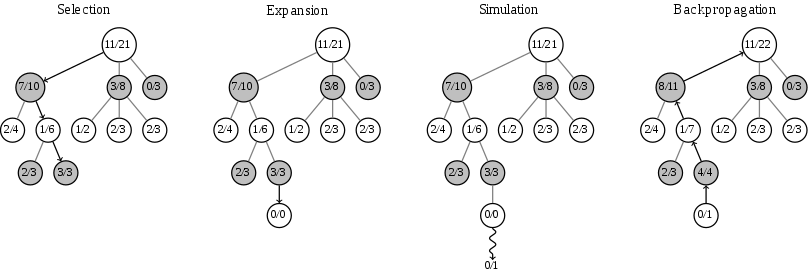
\includegraphics[scale=0.4]{./images/mcts.png}
  \centering
  \caption{Fazy algorytmu MCTS.\newline Źródło:\,\url{https://upload.wikimedia.org/wikipedia/commons/6/62/MCTS\_\%28English\%29\_-\_Updated\_2017-11-19.svg}}
  \label{fig:mcts}
\end{figure}


\subsection{Selection}
Jak sama nazwa wskazuje -- w kroku tym algorytm musi wybrać liść z aktualnego drzewa gry.
Na wybranym wierzchołku kolejno będzie wykonywana faza Expansion.
Poniżej pokazany jest przykładowa implementacja tego kroku wraz ze szczegółowym omówieniem (pseudocode).

\lstinputlisting{./mctsselection.pseudocode}

W powyższym kodzie w pierwszych wierszach jest zwracany węzeł, jeśli od korzenia drzewa dotarliśmy do liścia lub półliścia (czyli taki wierzchołek, w którym istnieją dzieci na których jeszcze nie była przeprowadzana faza symulacji).

W kolejnych liniach znajduje się funkcja eval\textunderscore func, która służy do oceny, w którą stronę idziemy dalej do liścia lub półliścia.
Funkcja ta jest warta uwagi dlatego poniżej znajduje się o nie trochę informacji.

\subsubsection{Trochę o eval\textunderscore func}
Funkcja ta ma pomóc wybrać wierzchołek z danej głębokości, który jest najbardziej obiecujący.
Dobrze jest, gdy wzór ten bierze pod uwagę liczbę wygranych oraz przeprowadzonych symulacji w danym wierzchołku.
Z powyższego powodu w pracy tej, jako eval\textunderscore func zaimplementowano wzór UCT:

\[ f\left(node\right) = \frac{node.wins}{node.simulations} + \alpha \cdot \sqrt{\frac{\ln{\left(all\_simulations\right)}}{node.simulations}} \]

\( \alpha \) to parametr, który według zaleceń równy jest \( \sqrt{2} \), w praktyce jego wartość dobierana jest podczas testów.

Zauważmy, że lewa strona sumy przyjmuje dużą wartość gdy w danym węźle jest dużo wygranych.
Prawa strona sumy z kolei przyjmuje duże wartości gdy w danym węźle przeprowadzono małą liczbę symulacji.
Przy takim przedstawieniu sumy widać, że parametr \( \alpha \) odpowiada za to co jest bardziej istotne przy wyborze kolejnego wierzchołka do ekspansji -- duża liczba wygranych, czy mała liczba przeprowadzonych symulacji w danym węźle.
W realnym świecie ta wartość jest zwykle dobierana na podstawie testów i symulacji -- co jest ważniejsze ekspansja, czy eksploatacja.

Następny w kolejności krok to Expansion -- opisany poniżej.

\subsection{Expansion}
Celem tego kroku jest rozbudowanie wierzchołka, który jest liściem lub półliściem.
Rozbudowanie, lub inaczej ekspansja, polega na rozbudowaniu kolejnego poziomu głębokości drzewa (z danego wierzchołka).

Poniżej zaprezentowano przykładową implementację tego kroku (pseudokod).

\lstinputlisting{./mctsexpansion.pseudocode}

W fazie selection wybrany wierzchołek jest liściem lub półliściem.
Przypadek liścia jest obsłużony w pierwszej kolejności -- inicjalizujemy dzieci węzła i wybieramy losowy niezainicjalizowany węzeł.
Przypadek półliścia to zwyczajny losowy wybór stanu-dziecka dla, którego symulacja nie była jeszcze przeprowadzona.

\subsection{Simulation}
W tym kroku symulujemy losową rozgrywkę z danego stanu do końca.
Poniżej, w pseudokodzie, przedstawiono przykładową implementację.

\lstinputlisting{./mctssimulation.pseudocode}

\subsection{Backpropagation}
W kroku tym aktualizujemy drzewo na podstawie wyniku uzyskanego w poprzednim kroku.

\lstinputlisting{./mctsback.pseudocode}

Jak widać w tej fazie algorytmu wchodzimy w górę drzewa aktualizując liczbę symulacji oraz wygranych.

Powyższe cztery kroki są powtarzane w kółko aż wykorzystają wyznaczony czas.
Po zakończeniu czasu przewidzianego na ruch zwracane jest dziecko korzenia (ruch), gdzie przeprowadzono największą liczbę symulacji (niekoniecznie ten, który miał największy współczynnik wygranych).
W ten sposób zapobiega się sytuacji gdy algorytm przeprowadził symulacje nowego stanu tuż przed przerwaniem pracy algorytmu.
Jest to ważne, ponieważ w przypadku wygranej nowego stanu będzie miał on współczynnik wygranych równy \( 1 \).

\subsubsection{Wady i zalety}
Wady:
\begin{itemize}
  \item Istnieją gry, w których losowa rozgrywka może trwać bardzo długo.
  \item Szczególnie przy małej liczbie symulacji, łatwo można otrzymać ruch nieoptymalny, niskiej jakości.
\end{itemize}
Zalety:
\begin{itemize}
  \item Łatwo ograniczyć czasowo jego wykonanie (przez odpowiednią liczbę symulacji)
  \item Nie wymaga heurystyki -- losowe rozgrywki spełniają tę rolę
  \item Dobrze nadaje się do gier trudnych, złożonych -- gdzie nie są znane dobre strategie (np. Go)
\end{itemize}

\section{Podsumowanie}
Powyżej zaprezentowano podstawowe wersje algorytmów.
Niemniej jednak algorytmy te można znacznie usprawnić -- poprzez liczne optymalizacji.
Część z tych optymalizacji można znaleźć w końcowej części pracy, dotyczącej propozycji usprawnień oraz dalszej rozbudowy oprogramowania.


\chapter{Omówienie biblioteki do pisania agentów}
W rozdziale tym zostało opisane wszystko co potrzebne, by nauczyć się używać oprogramowania napisanego na potrzeby tej pracy.
\section{Środowisko pisania modułu}
Podczas pisania biblioteki użyto:
\begin{itemize}
  \item System operacyjny -- Ubuntu 18.04
  \item Python 3.6.7 wraz ze standardowymi modułami oraz colorama.
\end{itemize}
\section{Co wchodzi w skład biblioteki}
W skład biblioteki wchodzi:
\begin{itemize}
  \item plik agent\textunderscore module.py -- jest to moduł do Pythona zawierający najważniejsze funkcje/klasy.
  \item plik game\textunderscore template.py -- jest to plik z szablonem gry planszowej mający na celu ułatwić projektowanie gry.
  \item ox.py, connect4.py, fox\textunderscore game.py, reversi.py -- przykłady tworzenia gier planszowych.
\end{itemize}


\section{Omówienie zasad przykładowych gier}
Poniżej zostały przedstawione zasady gier, które są zaimplementowane jako przykłady.
\subsection{Kółko i krzyżyk}
Gra odbywa się na planszy 3x3.
Jeden gracz umieszcza na planszy kółka, drugi zaś krzyżyki.
Gracze wykonują ruchy naprzemiennie. Celem gry jest ułożenie, jako pierwszy, trzech pionków w pionie, poziomie lub na skosie.
Rysunku \ref{fig:oxwin} przedstawia zakończoną grę.
Zwycięzcą jest gracz stawiający kółka.

\begin{figure}[H]
  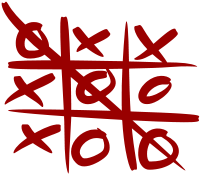
\includegraphics{./images/tictactoe.png}
  \centering
  \caption{Kółko i krzyżyk.\newline Źródło:\,\url{https://upload.wikimedia.org/wikipedia/commons/3/32/Tic\_tac\_toe.svg}}
  \label{fig:oxwin}
\end{figure}

Przykładowa implementacja tej gry znajduje się w pliku ox.py.
Kod programu do tej gry został też szczegółowo omówiony w dalszej części tej pracy.

\subsection{Connect Four}
W grze o nazwie Connect Four celem gracza jest takie ułożenie na planszy, żeby 4 jego pionki były połączone, podobnie jak w grze kółko i krzyżyk, w pionie, poziomie lub skosie.
Gracze wrzucają swoje pionki naprzemiennie od góry planszy.
Rysunki \ref{fig:c4} oraz \ref{fig:c4_2} przedstawiają przykładowy zestaw do gry w connect four -- pionowa plansza z otworami na górze -- do wrzucania pionków.

\begin{figure}[H]
  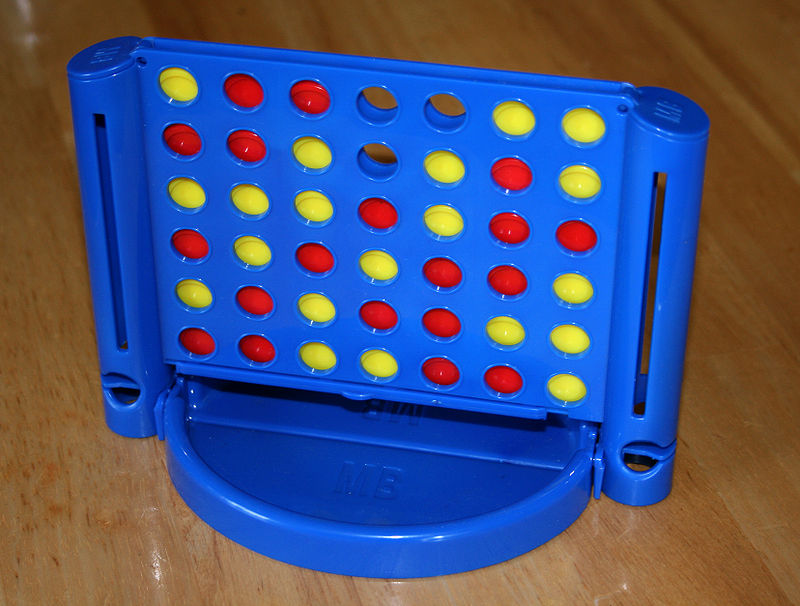
\includegraphics[scale=0.25]{./images/connect4.jpg}
  \centering
  \caption{Connect Four, Zakończona gra. \newline Źródło:\,\url{https://upload.wikimedia.org/wikipedia/commons/2/2a/Connect\_Four.jpg}}
  \label{fig:c4}
\end{figure}
\begin{figure}[H]
  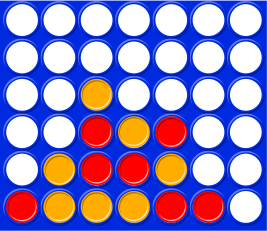
\includegraphics[scale=0.5]{./images/connect4.png}
  \centering
  \caption{Connect Four, W trakcie gry. \newline Źródło:\,\url{https://upload.wikimedia.org/wikipedia/commons/d/dc/Puissance4\_01.svg}}
  \label{fig:c4_2}
\end{figure}

Na rysunku \ref{fig:c4_2} widać grę, która jeszcze nie jest skończona.
Ruch ma gracz zaczynający. Na potrzeby tłumaczenia załóżmy, że ruch ma teraz gracz czerwony.
Zgodnie z zasadami może on wybrać dowolną kolumnę i wrzucić tam swój pionek.
Zarówno gracz żółty jak i czerwony, mają po 3 pionki ułożone na skosie, które mogą spróbować ułożyć na wygraną (4 pionki na skos).


\subsection{Lis i Gęsi}
Tutaj zostanie omówiony podstawowy wariant gry -- z jednym lisem i trzynastoma gęsiami.
Jest to prosta gra dwuosobowa. Jeden gracz porusza Lisem, drugi gęsiami.
Gra toczy się na planszy w kształcie krzyża.
Celem Lisa jest zbicie takiej liczby gęsi, by nie mogły one wygrać (przyjmuje się, że 8 zbitych gęsi jest wystarczające dla wygranej lisa).
Lis potrafi się poruszać po planszy oraz bić gęsi na takich samych zasadach jak w warcabach -- potrafi wykonać jedno lub więcej bić na skos do przodu i do tyłu. Bicie, tak samo jak w warcabach, wykonuje się przeskakując pionek lub pionki przeciwnika (gęsi).
Celem Gęsi jest uwięzienie lisa -- doprowadzenie do takiej sytuacji, że lis nie może się ruszyć ani zbić gęsi.
Gęsi w odróżnieniu od lisa mogą się tylko przemieszczać na sąsiednie wolne pola.
Grę rozpoczynają gęsi.
Rysunek \ref{fig:fg} przedstawia wariant gry z dwoma lisami i większą liczbą gęsi.
\begin{figure}[H]
  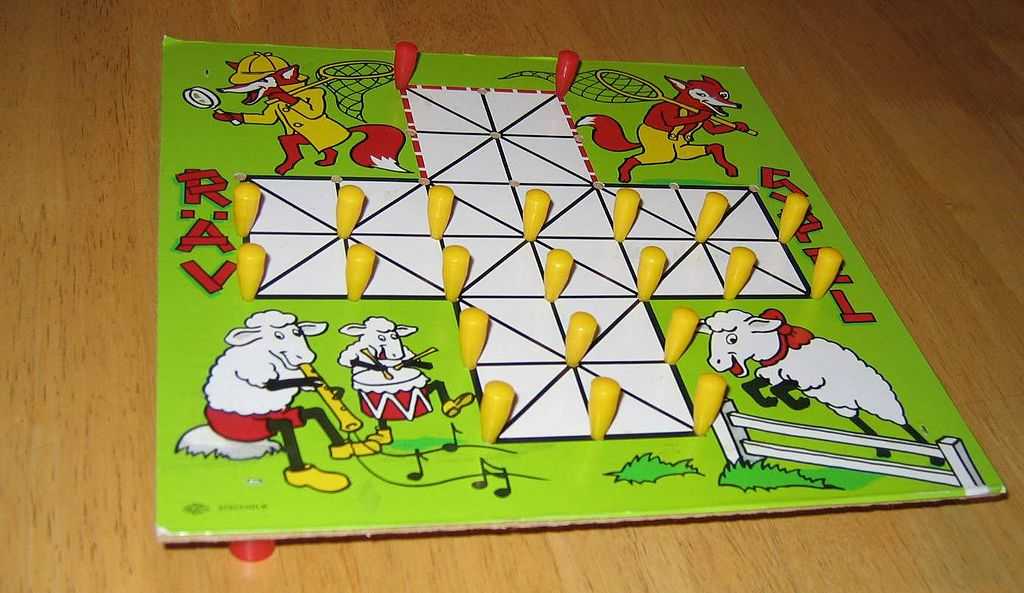
\includegraphics[scale=0.25]{./images/foxgames.jpg}
  \centering
  \caption{Fox Games.\newline Źródło:\,\url{https://upload.wikimedia.org/wikipedia/commons/d/d9/The\_fox\_game.jpg}}
  \label{fig:fg}
\end{figure}

Przykładowa implementacja tej gry znajduje się w pliku fox\textunderscore game.py

\subsection{Reversi}
Kolejną i ostatnią grą implementowaną na potrzeby tej pracy jest gra o nazwie reversi.
Gra odbywa się na planszy 8x8.
W grze tej jest dwóch graczy wykonujących swoje ruchy naprzemiennie.
Gracz zaczynający gra pionkami czarnymi, drugi gracz gra pionkami białymi.
Jeżeli któryś z graczy nie może wykonać poprawnego ruchu, wtedy traci turę.
Gra kończy się, gdy żaden z graczy nie może wykonać poprawnego ruchu.
Jeśli gracz chce wygrać powinien na zakończenie gry mieć więcej własnych pionków niż przeciwnik.

Teraz zostanie omówiony prawidłowy sposób wykonywania tury.
Jedyny ruch jaki można w tej grze wykonywać to dokładanie pionka.
Dokładanie pionka może odbywać się tylko w taki sposób, że tworzy linię (poziomą, pionową lub ukośną) z innym swoim pionkiem na początku (na drugim końcu linii), a pionkiem/ami przeciwnika pomiędzy (pomiędzy początkiem a pionkiem dołożonym mogą i muszą znajdować się tylko pionki przeciwnika).
Pionki przeciwnika znajdujące się na tej linii zmieniają kolor na kolor pionków gracza dokładającego.
W oczywisty sposób jednym ruchem można utworzyć więcej niż jedną taką linię -- co bywa korzystne.
Rysunki \ref{fig:reversi} oraz \ref{fig:reversi_moves} przedstawiają kolejno, stan początkowy oraz możliwe ruchy.
\begin{figure}[H]
  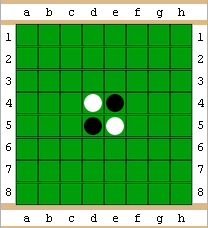
\includegraphics{./images/reversi.png}
  \centering
  \caption{Reversi, stan początkowy.\newline Źródło:\,\url{https://en.wikipedia.org/wiki/Reversi\#Rules}}
  \label{fig:reversi}
\end{figure}

\begin{figure}[H]
  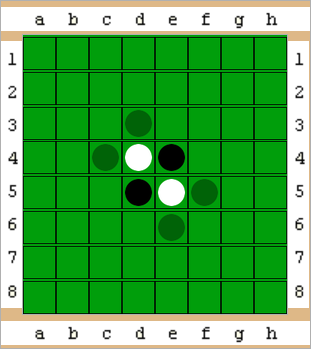
\includegraphics[scale=0.66]{./images/reversi_moves.png}
  \centering
  \caption{Reversi, W kolorze szarym oznaczono możliwe do wykonania ruchy czarnych pionków.\newline Źródło:\,\url{https://en.wikipedia.org/wiki/Reversi\#Rules}}
  \label{fig:reversi_moves}
\end{figure}

Przykładowa implementacja tej gry znajduje się w pliku reversi.py


\section{Omówienie szablonu gier planszowych}
Swoją pracę z omawianą biblioteką powinno się zacząć od zrozumienia pliku game\textunderscore template.py.
Na wstępie warto powiedzieć, że prawidłowe korzystanie z tego pliku polega na skopiowaniu go oraz poprawnym wyedytowaniu na potrzeby nowej gry.

\subsection{class GameTemplate}
W pliku tym znajduje się klasa GameTemplate.
Jest to najważniejsza część tego pliku.
Jak można zauważyć, klasa ta zawiera wiele metod -- nazwy tych metod nie powinny być zmieniane, ponieważ agent\textunderscore module.py korzysta z nich w swoich funkcjach.
Klasa ta to abstrakcyjny model gry planszowej -- zawierający wszystkie niezbędne funkcje -- które powinno się zaimplementować.

\subsection{Przykładowe AI}
W tym samym pliku, poniżej wcześniej wspomnianej klasy -- można znaleźć klasę NPCPlayer. Ten przykład jest bardzo prosty -- jest to zwykły agent grający losowo.
W tym miejscu warto wspomnieć, że nasz moduł do agentów wykorzystuje pole player\textunderscore id -- powinien być to unikatowy id dla agenta -- niekoniecznie to musi być, jak w przykładzie, jego pionek.
Niemniej jednak na potrzeby funkcji z agenta to pole powinno być zapewnione.

Na końcu tego pliku widać dwie linijki kodu, które odpowiadają za inicjalizacje oraz uruchomienie gry.
\section{Propozycja implementowania gier planszowych}
Dla ułatwienia pisania programu oraz szybkiego zapoznania się z biblioteką warto omówić rutynowe czynności, które występują przy pracy z omawianą biblioteką.
Poniżej omówione są dwie zawsze występujące, rutynowe, czynności.
\subsection{Tworzenie gry planszowej}
Tworzenie gry planszowej przy pomocy tej biblioteki sprowadza się do:
\begin{itemize}
  \item zmiany nazwy klasy GameTemplate na nazwę gry,
  \item implementacji logiki gry w metodach tej klasy (zgodnie z komentarzami),
  \item implementacji interfejsu graficznego gry,
  \item testowania programu.
\end{itemize}

\subsection{Tworzenie Agenta}
Tworzenie agenta w abstrakcyjnym ujęciu sprowadza sie do:
\begin{itemize}
  \item zmiany nazwy klasy agenta z pliku game\textunderscore template.py,
  \item utworzenia funkcji do oceny gry (jeśli potrzebna),
  \item poprawne wywołanie konstruktora klasy AgentAI,
  \item zapisanie logiki agenta w metodzie make\textunderscore move.
\end{itemize}

\section{Opis agent\textunderscore module.py}
Plik agent\textunderscore module.py to tytułowy moduł, który ma ułatwiać pisanie sztucznej inteligencji do gier planszowych.
Warte omówienia (ze względu na użycie) są trzy klasy, które się tutaj znajdują:
\begin{itemize}
  \item GameBoard
  \item AgentAI
  \item HumanPlayer
\end{itemize}

\subsection{Klasa GameBoard}
Klasa GameBoard zawiera metody takie jak:
\begin{itemize}
  \item is\textunderscore on\textunderscore board -- zwraca prawdę jeżeli dane współrzędne leżą na planszy -- fałsz w przeciwnym wypadku.
  \item count\textunderscore symbol -- zwraca liczbę wystąpienia znaku na planszy.
  \item is\textunderscore unoccupied -- odpowiada na pytanie czy dane pole jest zajęte.
  \item is\textunderscore occupied -- logiczna negacja poprzedniej metody.
  \item print\textunderscore board -- funkcja do wypisywania w konsoli (znakami ascii -- colorama) planszy do gry.
  Funkcja jest domyślnie skonfigurowana i nie potrzebuje parametrów.
\end{itemize}
Sposoby użycia tej klasy są dobrze widoczne w dołączonych przykładowych grach np. reversi.py.

\subsection{Klasa AgentAI}
Klasa AgentAI zawiera pola i metody -- poniżej przedstawiono ważniejsze z nich.
Ważniejsze pola uzywane w funkcji init:
\begin{itemize}
  \item player\textunderscore id -- unikatowe id gracza -- służy do jego identyfikacji
  \item game\textunderscore heuristic -- funkcja oceniająca stan gry -- domyślna heurystyka symuluje losowe rozgrywki i na tej podstawie ocenia.
  \item max\textunderscore depth -- maksymalna głębokość budowanego drzewa dla funkcji takich jak MiniMax etc. Domyślna wartość to \( +\infty \)
  \item number\textunderscore simulations -- liczba symulacji dla funkcji takich jak mcts etc. Zmienna ta jest używana także dla domyślnej heurystyki -- mówi ile razy wykonać symulację zanim heurystyka zwróci wynik. Domyślna wartość to 10.
\end{itemize}

Poniżej znajdują się ważniejsze metody używane w klasie agenta.
Wszystkie poniższe funkcje mają jeden parametr -- jest to aktualna gra (obiekt implementujący metody podane w klasie GameTemplate).
\begin{itemize}
  \item minimax\textunderscore move -- funkcja zwraca ruch wybrany metodą MiniMax.
  \item random\textunderscore move -- funkcja zwraca losowy ruch.
  \item alpha\textunderscore beta\textunderscore move -- funkcja zwraca ruch wybrany algorytmem Alpha-Beta.
  \item mcts\textunderscore move -- funkcja zwraca ruch wybrany przez algorytm Monte Carlo Tree Search.
  Prametry startowe (np. liczba symulacji) konfigurowane są podczas inicjalizacji agenta (np. number\textunderscore simulations).
\end{itemize}
Przykłady użycia również widoczne są w przykładowych grach np. fox\textunderscore game.py

\subsection{Klasa HumanPlayer}
Klasa HumanPlayer została zaimplementowana jako pomoc przy debugowaniu.
Jej celem jest zapewnienie minimalnej wizualizacji możliwych ruchów oraz możliwość wybrania go przez człowieka.
Klasy ta dziedziczy po AgentAI, a co więcej jest używana tak jak inni gracze w przykładowych programach.
Dla przykładu znaczy to, że aby zagrać w grę kółko i krzyży wystarczy w pliku ox.py linię:
\lstinputlisting[firstline=97,lastline=97,firstnumber=97]{../ox.py}
zamienić na:
\lstinputlisting[firstnumber=95]{humanplayer}
uprzednio importując z tego modułu klasę HumanPlayer.

\section{Omówienie kodu do gry w kółko i krzyżyk}
Na potrzeby omówienia tej pracy wybrano grę w kółko i krzyżyk.
Sama gra nie jest w żaden sposób interesująca.
Grę tą wybrano jedynie ze względu na prostotę logiki oraz zwięzłość kodu -- możliwego do umieszczenia w tejże pracy.
\subsection{Kod gry kółko i krzyżyk}
\lstinputlisting{../ox.py}
\subsection{Wytłumaczenie powyższego kodu}
Na początku widać klasę OX. Jest to klasa GameTemplate ze zmienioną nazwą.
Kolejno w liniach 4-11 widać inicjalizację klasy (konstruktor):
\lstinputlisting[firstline=4,lastline=11,firstnumber=4]{../ox.py}
Warto zwrócić uwagę, że na samym początku tworzymy pustą planszę do gry w kółko i krzyżyk.
Kropki na naszej planszy oznaczają pola wolne.
Klasa GameBoard przyjmuje jako parametr planszę do gry (w dowolnym formacie) oraz listy symboli dla graczy -- potrzebne dla funkcji print\textunderscore board.
W przypadku naszej gry jej użycie nie jest konieczne -- korzystamy tylko z funkcji do rysowania planszy.
Sama ta klasa zapewnia najbardziej podstawowe funkcje do debugowania i wspomagające operacje na planszach typu tablica dwuwymiarowa.

Kolejna metoda klasy OX to get\textunderscore opponent
\lstinputlisting[firstline=13,lastline=17,firstnumber=13]{../ox.py}
Metoda ta ma na celu podanie przeciwnika dla podanego w parametrze gracza.
Jest to funkcja z której korzystają algorytmy takie jak alpha-beta, minimax -- stąd potrzeba jej implementacji.
Pomimo tego, że powyższa funkcja jest trywialna -- postanowiono o niej jednak wspomnieć, ponieważ niektóre gry można zaimplementować np. z trójką graczy (MCTS powinien sobie poradzić z wersją kółka i krzyżyka dla trzech graczy).

Dalej można znaleźć metody dwie kolejne metody wymagane przez bibliotekę:
\lstinputlisting[firstline=19,lastline=26,firstnumber=19]{../ox.py}

Pierwsza z tych funkcji get\textunderscore allowed\textunderscore moves powinna zwracać wszystkie możliwe ruchy dla danego gracza.
Format odpowiedzi to powinna być tablica ruchów właśiwie w dowolnym formacie, który jest rozumiany przez funkcję apply\textunderscore move.
W naszym wypadku gracz nie ma znaczenia, ponieważ możliwe ruchy to wolne pola na planszy (i nie zależy to od gracza).
Funkcja ta przyjmuje gracza jako argument tylko dla wymagań biblioteki.
Obydwie te funkcje są potrzebne do poprawnego działania algorytmów przeszukiwania.

Ostatnie dwie ważne funkcje to is\textunderscore winner oraz game\textunderscore end.
Pierwsza z nich odpowiada, czy gracz podany jako argument jest zwycięzcą gry (jeśli gra się zakończyła), druga odpowiada na pytanie czy gra jest zakończona.
Podobnie jak wyżej te funkcje są potrzebne dla wyżej wymienionych algorytmów i implementują logikę właściwą dla konkretnej gry.

Pozostała część kodu to funkcjonalności potrzebne do działania gry, stworzone w sposób opisany w poprzednim punkcie tego rozdziału.

\section{Pozostałe gry}
Pozostałe gry ze względu na swoje rozmiary nie zostały w tej pracy szczegółowo opisane.
Jednak zostaną one teraz pokrótce przedstawione.

\subsection{connect4.py}
Implementacja do gry w connect four znajduje się w pliku connect4.py
W pliku tym najbardziej niestandardową rzeczą jaka się znajduje, jest dostosowywanie funkcji print\textunderscore board.
Dostosowanie kolorów polega na stworzeniu niebieskiej planszy, oraz zadbanie o to by pionki graczy były w kolorach czerwonych i żółtych.
Agenci, którzy tutaj grają to zwykli agenci grający losowo -- wykorzystujący funkcję random\textunderscore move.
Rysunek \ref{fig:c4_game} przedstawia zrzut ekranu z zakończonej rozgrywki.
Wygrał gracz nr 2 -- grający pionkami żółtymi.

\begin{figure}[H]
  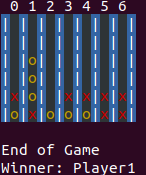
\includegraphics{./images/connect4game.png}
  \centering
  \caption{Connect Four -- zakończona gra.}
  \label{fig:c4_game}
\end{figure}


\subsection{fox\textunderscore game.py}
Implementacja do gry Lis i Gęsi znajduje się w pliku fox\textunderscore game.py.
Warto tutaj zauważyć, że plansza jest niestandardowa -- duża oraz kwadratowa.
Zaimplementowano dwóch agentów -- jeden dla gęsi, drugi dla lisa.
Agent grający Gęsiami, gra losowo.
Agent grający Lisem, jeśli ma ruch typu bicie, wtedy wykonuje maksymalne możliwe bicie (bije maksymalną możliwą ilość gęsi).
Jeśli Lis nie ma dostępnego ruchu typu bicie -- gra ruch alpha-beta z domyślną heurystyką.
Z tego powodu zwykle wygrywa lis.
Rysunek \ref{fig:fox_start} przedstawia wygląd stanu początkowego.
Jak widać plansza jest zbyt duża by można było ponumerować kolumny liczbami jednocyfrowymi -- dlatego górna etykieta składa się z dwóch wierszy.

\begin{figure}[H]
  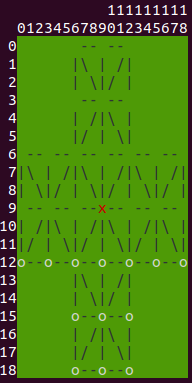
\includegraphics[scale=0.5]{./images/foxstartgame.png}
  \centering
  \caption{Fox Games -- stan początkowy.}
  \label{fig:fox_start}
\end{figure}

\subsection{reversi.py}

Implementacja do gry reversi znajduje się w pliku reversi.py.
W pliku tym jedyną niestandardową rzeczą jest napisana heurystyka do algorytmu Alpha-Beta.
Heurystyka ta przypisuje wagi poszczególnym polom -- np. najwięcej warte są pola w rogach.
Rysunek \ref{fig:rev_wag} przedstawia wagi poszczególnych pól na planszy do reversi.
\begin{figure}[H]
  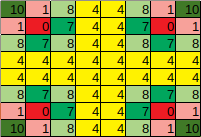
\includegraphics[scale=0.8]{./images/revwag.png}
  \centering
  \caption{Reversi -- wagi poszczególnych pól.}
  \label{fig:rev_wag}
\end{figure}

Jak widać najwięcej warte są pola na rogach, ponieważ te pola są pewne (nie da się zbić pionka w rogu).
Najmniej warte są pola, które ułatwiają przeciwnikowi zajęcie pola w rogu.
Gracz alpha-beta domyślnie ma ograniczenie głębokości do 7.

Drugi agent korzysta z algorytmu MCTS (300 symulacji na ruch) -- liczba symulacji została dobrana eksperymentalnie -- tak żeby ruch gracza mcts zajmował w przybliżeniu tyle samo czasu co ruch gracz alpha-beta.

Na 10 przeprowadzonych gier gracz grający Alpha-Beta przegrał wszystkie partie.
Dzieje się tak dlatego, że zajmowanie poszczególnych pól nie jest najlepszą taktyką -- gra w reversi jest bardzo dynamiczna -- tymczasowy zwycięzca często się zmienia.
To zdarzenie dobrze widać na rysunku \ref{fig:rev_mid}, gdzie gracz MCTS ma bardzo mało pionków (gracz x), a na zakończeniu (Rys. \ref{fig:rev_end}) gry, widać bezpieczną wygraną, gracza MCTS.
Na poniższych rysunkach widać zrzuty ekranu z poszczególnych etapów gry.


\begin{figure}[H]
  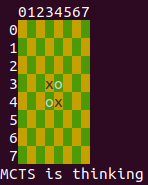
\includegraphics[scale=0.8]{./images/reversistart.png}
  \centering
  \caption{Reversi -- stan początkowy.}
  \label{fig:rev_start}
\end{figure}

\begin{figure}[H]
  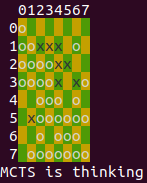
\includegraphics[scale=0.8]{./images/reversimid.png}
  \centering
  \caption{Reversi -- MCTS vs Alpha-Beta -- W trakcie gry.}
  \label{fig:rev_mid}
\end{figure}

\begin{figure}[H]
  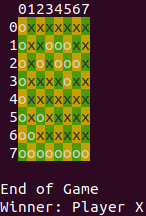
\includegraphics[scale=0.8]{./images/reversiend.png}
  \centering
  \caption{Reversi -- MCTS vs Alpha-Beta -- koniec gry.}
  \label{fig:rev_end}
\end{figure}

Jednak wystarczy by algorytm MCTS przeprowadzał małą liczbę symulacji (np. 100) i już nie jest w stanie wygrać (gracz alpha-beta gra końcówki bez heurystyki).

\section{Propozycje dalszego rozwoju biblioteki}
\subsection{Propozycje rozbudowy oprogramowania}
Poniżej przedstawiono propozycje rozbudowy oprogramowania.
Propozycje te wykraczają poza tematyke pracy, jednak ze względu na ich wartościowość, zostały one tutaj zamieszczone.
\begin{itemize}
  \item Dodanie innych algorytmów przeszukiwania (bez adwersarza) (A*, DFS, BFS (głównie z myślą o celach edukacyjnych))
  \item Przemyślenia wsparcia dla sieci neuronowych i deep learningu.
  \item Przeprowadzenie benchmarków i porównanie wykonywania poszczególnych programów w Cythonie\cite{cython} oraz PyPy\cite{pypy} -- zadbanie o to by dalsza rozbudowa była zgodna z najszybszą implementacją języka Python.
  \item Dodanie testów automatycznych -- zadbanie o to by wprowadzanie nowych zmian można było łatwo testować. Szczególnie należy zadbać by podstawowe algorytmy posiadały testy.
\end{itemize}

\subsection{Propozycje optymalizacji i usprawnień}
Poniżej przedstawiono propozycje usprawnień już zaimplementowanych algorytmów.

\subsubsection{Optymalizacje i usprawnienia algorytmu Alpha-Beta i MiniMax}
Implementowane wersje algorytmu Alpha-Beta oraz Mini-Max są podstawowymi wersjami tych algorytmów.
Stąd możliwe są usprawnienia takie jak:
\begin{itemize}
  \item Jak już wspomniano, algorytm Alpha-Beta działa szybciej gdy przegląda ruchy w kolejności uporządkowanej.
    Ze względu na ten fakt, zanim algorytm zacznie iterację po liście zawierającym dzieci, listę tą można uporządkować, używając do porównania funkcji oceniającej.
    Zakłada się, że nawet bardzo prosta heurystyka powinna zauważalnie przyśpieszyć działanie algorytmu.
  \item zwykły algorytm MiniMax można wykonywać wielowątkowo -- analiza poszczególnych ruchów jest od siebie niezależna, stąd nic nie stoi na przeszkodzie aby analizę poszczególnych ruchów prowadziły, równolegle, różne wątki.
\end{itemize}

\subsubsection{Optymalizacje i usprawnienia algorytmu MCTS}
Implementowana wersja algorytmu Monte Carlo Tree Search jest również podstawową wersją algorytmu.
Stąd przykładowe optymalizacje to:

\begin{itemize}
  \item Zanim przejdziemy do rozbudowywania drzewa, bezsensowne ruchy można z góry odrzucić.
  \item Dla dobrych ruchów, np. ruchy wygrywające, lub wygrywające w paru ruchach (możliwe do oceny przez prostą heurystykę), można zwiększać wartość funkcji przedstawionej w pseudokodzie jako eval\textunderscore func (funkcja wybiera kolejny wierzchołek z drzewa gry do rozbudowywania/symulacji). Taka pozornie drobna zmiana spowoduje, że algorytm będzie więcej czasu spędzał w potencjalnie dobrych ruchach.
  \item Algorytm MCTS idealnie nadaje się do bycia wspartym przez wielowątkowość -- w taki sam sposób jak w przypadku algorytmu Mini-Max.
\end{itemize}

\chapter{Zakończenie}
Głównym celem pracy było dostarczenie oprogramowania pomocnego w tworzeniu sztucznej inteligencji do gier planszowych.
Jak widać cel pracy został osiągnięty -- powstała biblioteka wspomagająca tworzenie inteligentnych agentów do gier planszowych.
Zaimplementowano także liczne przykłady użycia biblioteki, zgodnie z zasadą, że dostęp do kodu jest często lepszy niż szczegółowa dokumentacja.
W obecnym stanie z biblioteki korzysta się przyjemnie do tworzenia zarówno gier planszowych jak i agentów do niej.
Biblioteka została napisana z dbałością o to, by zapewnić łatwość jej przyszłej rozbudowy.
Zadbano także by liczne propozycje usprawnień oraz dalszej rozbudowy oprogramowania znajdowały sie w tej pracy.


%%%%% BIBLIOGRAFIA

\begin{thebibliography}{1}

\bibitem{aibook} Stuart Russell, Peter Norvig. Artificial Intelligence: A Modern Approach. Pearson; 3 edition (December 11, 2009).

\bibitem{wazniak} Lekcja ze sztucznej inteligencji [online]. Artykuł dostępny w internecie:\newline
\url{http://wazniak.mimuw.edu.pl/index.php?title=Sztuczna_inteligencja/SI_Modu%C5%82_8_-_Gry_dwuosobowe}

\bibitem{mcts1} Michele Sebag, Monte-Carlo Tree Search [online]. Wykład dostępny w internecie:\newline
\url{https://www.lri.fr/~sebag/Slides/InvitedTutorial\_CP12.pdf}

\bibitem{deepblue} DeepBlue -- komputer od firmy IBM [online]. Artykuł dostępny w internecie:\newline
\url{https://www.ibm.com/ibm/history/ibm100/us/en/icons/deepblue/}

\bibitem{alphago} AlphaGo -- Deepmind [online]. Artykuł dostępny w internecie:\newline
\url{https://deepmind.com/research/alphago/}

\bibitem{cython} Cython -- oficjalna strona projektu [online]
\url{https://cython.org/}

\bibitem{pypy} PyPy -- oficjalna strona projektu [online]
\url{https://pypy.org/}

\bibitem{python} Python -- oficjalna strona projektu [online]
\url{https://www.python.org/}


\end{thebibliography}

\end{document}
